\documentclass[a4paper,12pt]{article}

	%\usepackage[latin1]{inputenc}
	\usepackage[portuguese]{babel}

    \usepackage[breakable]{tcolorbox}
    \usepackage{parskip} % Stop auto-indenting (to mimic markdown behaviour)
    \usepackage{textgreek}

    
    
    \usepackage{iftex}
    \ifPDFTeX
    	\usepackage[T1]{fontenc}
    	\usepackage{mathpazo}
    \else
    	\usepackage{fontspec}
    \fi

    % Basic figure setup, for now with no caption control since it's done
    % automatically by Pandoc (which extracts ![](path) syntax from Markdown).
    \usepackage{graphicx}
    % Maintain compatibility with old templates. Remove in nbconvert 6.0
    \let\Oldincludegraphics\includegraphics
    % Ensure that by default, figures have no caption (until we provide a
    % proper Figure object with a Caption API and a way to capture that
    % in the conversion process - todo).
    \usepackage[justification=centering]{caption}
    %\DeclareCaptionFormat{nocaption}{}
    \captionsetup{aboveskip=0pt,belowskip=0pt}

    \usepackage{float}
    \floatplacement{figure}{H} % forces figures to be placed at the correct location
    \floatplacement{table}{H} % forces tables to be placed at the correct location
    \usepackage{xcolor} % Allow colors to be defined
    \usepackage{enumerate} % Needed for markdown enumerations to work
    \usepackage{geometry} % Used to adjust the document margins
    \usepackage{amsmath} % Equations
    \usepackage{amssymb} % Equations
    \usepackage{textcomp} % defines textquotesingle
    % Hack from http://tex.stackexchange.com/a/47451/13684:
    \AtBeginDocument{%
        \def\PYZsq{\textquotesingle}% Upright quotes in Pygmentized code
    }
    \usepackage{upquote} % Upright quotes for verbatim code
    \usepackage{eurosym} % defines \euro
    \usepackage[mathletters]{ucs} % Extended unicode (utf-8) support
    \usepackage{fancyvrb} % verbatim replacement that allows latex
    \usepackage{grffile} % extends the file name processing of package graphics 
                         % to support a larger range
    \makeatletter % fix for old versions of grffile with XeLaTeX
    \@ifpackagelater{grffile}{2019/11/01}
    {
      % Do nothing on new versions
    }
    {
      \def\Gread@@xetex#1{%
        \IfFileExists{"\Gin@base".bb}%
        {\Gread@eps{\Gin@base.bb}}%
        {\Gread@@xetex@aux#1}%
      }
    }
    \makeatother
    \usepackage[Export]{adjustbox} % Used to constrain images to a maximum size
    \adjustboxset{max size={0.9\linewidth}{0.9\paperheight}}

    % The hyperref package gives us a pdf with properly built
    % internal navigation ('pdf bookmarks' for the table of contents,
    % internal cross-reference links, web links for URLs, etc.)
    \usepackage{hyperref}
    % The default LaTeX title has an obnoxious amount of whitespace. By default,
    % titling removes some of it. It also provides customization options.
    \usepackage{titling}
    \usepackage{longtable} % longtable support required by pandoc >1.10
    \usepackage{booktabs}  % table support for pandoc > 1.12.2
    \usepackage[inline]{enumitem} % IRkernel/repr support (it uses the enumerate* environment)
    \usepackage[normalem]{ulem} % ulem is needed to support strikethroughs (\sout)
                                % normalem makes italics be italics, not underlines
    \usepackage{mathrsfs}
    

    
    % Colors for the hyperref package
    \definecolor{urlcolor}{rgb}{0,0,0} %{0,0,0.5} é azul escuro
    \definecolor{linkcolor}{rgb}{0,0,0}
    \definecolor{citecolor}{rgb}{0,0,0}

    % ANSI colors
    \definecolor{ansi-black}{HTML}{3E424D}
    \definecolor{ansi-black-intense}{HTML}{282C36}
    \definecolor{ansi-red}{HTML}{E75C58}
    \definecolor{ansi-red-intense}{HTML}{B22B31}
    \definecolor{ansi-green}{HTML}{00A250}
    \definecolor{ansi-green-intense}{HTML}{007427}
    \definecolor{ansi-yellow}{HTML}{DDB62B}
    \definecolor{ansi-yellow-intense}{HTML}{B27D12}
    \definecolor{ansi-blue}{HTML}{208FFB}
    \definecolor{ansi-blue-intense}{HTML}{0065CA}
    \definecolor{ansi-magenta}{HTML}{D160C4}
    \definecolor{ansi-magenta-intense}{HTML}{A03196}
    \definecolor{ansi-cyan}{HTML}{60C6C8}
    \definecolor{ansi-cyan-intense}{HTML}{258F8F}
    \definecolor{ansi-white}{HTML}{C5C1B4}
    \definecolor{ansi-white-intense}{HTML}{A1A6B2}
    \definecolor{ansi-default-inverse-fg}{HTML}{FFFFFF}
    \definecolor{ansi-default-inverse-bg}{HTML}{000000}

    % common color for the border for error outputs.
    \definecolor{outerrorbackground}{HTML}{FFDFDF}

    % commands and environments needed by pandoc snippets
    % extracted from the output of `pandoc -s`
    \providecommand{\tightlist}{%
      \setlength{\itemsep}{0pt}\setlength{\parskip}{0pt}}
    \DefineVerbatimEnvironment{Highlighting}{Verbatim}{commandchars=\\\{\}}
    % Add ',fontsize=\small' for more characters per line
    \newenvironment{Shaded}{}{}
    \newcommand{\KeywordTok}[1]{\textcolor[rgb]{0.00,0.44,0.13}{\textbf{{#1}}}}
    \newcommand{\DataTypeTok}[1]{\textcolor[rgb]{0.56,0.13,0.00}{{#1}}}
    \newcommand{\DecValTok}[1]{\textcolor[rgb]{0.25,0.63,0.44}{{#1}}}
    \newcommand{\BaseNTok}[1]{\textcolor[rgb]{0.25,0.63,0.44}{{#1}}}
    \newcommand{\FloatTok}[1]{\textcolor[rgb]{0.25,0.63,0.44}{{#1}}}
    \newcommand{\CharTok}[1]{\textcolor[rgb]{0.25,0.44,0.63}{{#1}}}
    \newcommand{\StringTok}[1]{\textcolor[rgb]{0.25,0.44,0.63}{{#1}}}
    \newcommand{\CommentTok}[1]{\textcolor[rgb]{0.38,0.63,0.69}{\textit{{#1}}}}
    \newcommand{\OtherTok}[1]{\textcolor[rgb]{0.00,0.44,0.13}{{#1}}}
    \newcommand{\AlertTok}[1]{\textcolor[rgb]{1.00,0.00,0.00}{\textbf{{#1}}}}
    \newcommand{\FunctionTok}[1]{\textcolor[rgb]{0.02,0.16,0.49}{{#1}}}
    \newcommand{\RegionMarkerTok}[1]{{#1}}
    \newcommand{\ErrorTok}[1]{\textcolor[rgb]{1.00,0.00,0.00}{\textbf{{#1}}}}
    \newcommand{\NormalTok}[1]{{#1}}
    
    % Additional commands for more recent versions of Pandoc
    \newcommand{\ConstantTok}[1]{\textcolor[rgb]{0.53,0.00,0.00}{{#1}}}
    \newcommand{\SpecialCharTok}[1]{\textcolor[rgb]{0.25,0.44,0.63}{{#1}}}
    \newcommand{\VerbatimStringTok}[1]{\textcolor[rgb]{0.25,0.44,0.63}{{#1}}}
    \newcommand{\SpecialStringTok}[1]{\textcolor[rgb]{0.73,0.40,0.53}{{#1}}}
    \newcommand{\ImportTok}[1]{{#1}}
    \newcommand{\DocumentationTok}[1]{\textcolor[rgb]{0.73,0.13,0.13}{\textit{{#1}}}}
    \newcommand{\AnnotationTok}[1]{\textcolor[rgb]{0.38,0.63,0.69}{\textbf{\textit{{#1}}}}}
    \newcommand{\CommentVarTok}[1]{\textcolor[rgb]{0.38,0.63,0.69}{\textbf{\textit{{#1}}}}}
    \newcommand{\VariableTok}[1]{\textcolor[rgb]{0.10,0.09,0.49}{{#1}}}
    \newcommand{\ControlFlowTok}[1]{\textcolor[rgb]{0.00,0.44,0.13}{\textbf{{#1}}}}
    \newcommand{\OperatorTok}[1]{\textcolor[rgb]{0.40,0.40,0.40}{{#1}}}
    \newcommand{\BuiltInTok}[1]{{#1}}
    \newcommand{\ExtensionTok}[1]{{#1}}
    \newcommand{\PreprocessorTok}[1]{\textcolor[rgb]{0.74,0.48,0.00}{{#1}}}
    \newcommand{\AttributeTok}[1]{\textcolor[rgb]{0.49,0.56,0.16}{{#1}}}
    \newcommand{\InformationTok}[1]{\textcolor[rgb]{0.38,0.63,0.69}{\textbf{\textit{{#1}}}}}
    \newcommand{\WarningTok}[1]{\textcolor[rgb]{0.38,0.63,0.69}{\textbf{\textit{{#1}}}}}
    
    
    % Define a nice break command that doesn't care if a line doesn't already
    % exist.
    \def\br{\hspace*{\fill} \\* }
    % Math Jax compatibility definitions
    \def\gt{>}
    \def\lt{<}
    \let\Oldtex\TeX
    \let\Oldlatex\LaTeX
    \renewcommand{\TeX}{\textrm{\Oldtex}}
    \renewcommand{\LaTeX}{\textrm{\Oldlatex}}
   
    
    
    
    
    
% Pygments definitions
\makeatletter
\def\PY@reset{\let\PY@it=\relax \let\PY@bf=\relax%
    \let\PY@ul=\relax \let\PY@tc=\relax%
    \let\PY@bc=\relax \let\PY@ff=\relax}
\def\PY@tok#1{\csname PY@tok@#1\endcsname}
\def\PY@toks#1+{\ifx\relax#1\empty\else%
    \PY@tok{#1}\expandafter\PY@toks\fi}
\def\PY@do#1{\PY@bc{\PY@tc{\PY@ul{%
    \PY@it{\PY@bf{\PY@ff{#1}}}}}}}
\def\PY#1#2{\PY@reset\PY@toks#1+\relax+\PY@do{#2}}

\expandafter\def\csname PY@tok@w\endcsname{\def\PY@tc##1{\textcolor[rgb]{0.73,0.73,0.73}{##1}}}
\expandafter\def\csname PY@tok@c\endcsname{\let\PY@it=\textit\def\PY@tc##1{\textcolor[rgb]{0.25,0.50,0.50}{##1}}}
\expandafter\def\csname PY@tok@cp\endcsname{\def\PY@tc##1{\textcolor[rgb]{0.74,0.48,0.00}{##1}}}
\expandafter\def\csname PY@tok@k\endcsname{\let\PY@bf=\textbf\def\PY@tc##1{\textcolor[rgb]{0.00,0.50,0.00}{##1}}}
\expandafter\def\csname PY@tok@kp\endcsname{\def\PY@tc##1{\textcolor[rgb]{0.00,0.50,0.00}{##1}}}
\expandafter\def\csname PY@tok@kt\endcsname{\def\PY@tc##1{\textcolor[rgb]{0.69,0.00,0.25}{##1}}}
\expandafter\def\csname PY@tok@o\endcsname{\def\PY@tc##1{\textcolor[rgb]{0.40,0.40,0.40}{##1}}}
\expandafter\def\csname PY@tok@ow\endcsname{\let\PY@bf=\textbf\def\PY@tc##1{\textcolor[rgb]{0.67,0.13,1.00}{##1}}}
\expandafter\def\csname PY@tok@nb\endcsname{\def\PY@tc##1{\textcolor[rgb]{0.00,0.50,0.00}{##1}}}
\expandafter\def\csname PY@tok@nf\endcsname{\def\PY@tc##1{\textcolor[rgb]{0.00,0.00,1.00}{##1}}}
\expandafter\def\csname PY@tok@nc\endcsname{\let\PY@bf=\textbf\def\PY@tc##1{\textcolor[rgb]{0.00,0.00,1.00}{##1}}}
\expandafter\def\csname PY@tok@nn\endcsname{\let\PY@bf=\textbf\def\PY@tc##1{\textcolor[rgb]{0.00,0.00,1.00}{##1}}}
\expandafter\def\csname PY@tok@ne\endcsname{\let\PY@bf=\textbf\def\PY@tc##1{\textcolor[rgb]{0.82,0.25,0.23}{##1}}}
\expandafter\def\csname PY@tok@nv\endcsname{\def\PY@tc##1{\textcolor[rgb]{0.10,0.09,0.49}{##1}}}
\expandafter\def\csname PY@tok@no\endcsname{\def\PY@tc##1{\textcolor[rgb]{0.53,0.00,0.00}{##1}}}
\expandafter\def\csname PY@tok@nl\endcsname{\def\PY@tc##1{\textcolor[rgb]{0.63,0.63,0.00}{##1}}}
\expandafter\def\csname PY@tok@ni\endcsname{\let\PY@bf=\textbf\def\PY@tc##1{\textcolor[rgb]{0.60,0.60,0.60}{##1}}}
\expandafter\def\csname PY@tok@na\endcsname{\def\PY@tc##1{\textcolor[rgb]{0.49,0.56,0.16}{##1}}}
\expandafter\def\csname PY@tok@nt\endcsname{\let\PY@bf=\textbf\def\PY@tc##1{\textcolor[rgb]{0.00,0.50,0.00}{##1}}}
\expandafter\def\csname PY@tok@nd\endcsname{\def\PY@tc##1{\textcolor[rgb]{0.67,0.13,1.00}{##1}}}
\expandafter\def\csname PY@tok@s\endcsname{\def\PY@tc##1{\textcolor[rgb]{0.73,0.13,0.13}{##1}}}
\expandafter\def\csname PY@tok@sd\endcsname{\let\PY@it=\textit\def\PY@tc##1{\textcolor[rgb]{0.73,0.13,0.13}{##1}}}
\expandafter\def\csname PY@tok@si\endcsname{\let\PY@bf=\textbf\def\PY@tc##1{\textcolor[rgb]{0.73,0.40,0.53}{##1}}}
\expandafter\def\csname PY@tok@se\endcsname{\let\PY@bf=\textbf\def\PY@tc##1{\textcolor[rgb]{0.73,0.40,0.13}{##1}}}
\expandafter\def\csname PY@tok@sr\endcsname{\def\PY@tc##1{\textcolor[rgb]{0.73,0.40,0.53}{##1}}}
\expandafter\def\csname PY@tok@ss\endcsname{\def\PY@tc##1{\textcolor[rgb]{0.10,0.09,0.49}{##1}}}
\expandafter\def\csname PY@tok@sx\endcsname{\def\PY@tc##1{\textcolor[rgb]{0.00,0.50,0.00}{##1}}}
\expandafter\def\csname PY@tok@m\endcsname{\def\PY@tc##1{\textcolor[rgb]{0.40,0.40,0.40}{##1}}}
\expandafter\def\csname PY@tok@gh\endcsname{\let\PY@bf=\textbf\def\PY@tc##1{\textcolor[rgb]{0.00,0.00,0.50}{##1}}}
\expandafter\def\csname PY@tok@gu\endcsname{\let\PY@bf=\textbf\def\PY@tc##1{\textcolor[rgb]{0.50,0.00,0.50}{##1}}}
\expandafter\def\csname PY@tok@gd\endcsname{\def\PY@tc##1{\textcolor[rgb]{0.63,0.00,0.00}{##1}}}
\expandafter\def\csname PY@tok@gi\endcsname{\def\PY@tc##1{\textcolor[rgb]{0.00,0.63,0.00}{##1}}}
\expandafter\def\csname PY@tok@gr\endcsname{\def\PY@tc##1{\textcolor[rgb]{1.00,0.00,0.00}{##1}}}
\expandafter\def\csname PY@tok@ge\endcsname{\let\PY@it=\textit}
\expandafter\def\csname PY@tok@gs\endcsname{\let\PY@bf=\textbf}
\expandafter\def\csname PY@tok@gp\endcsname{\let\PY@bf=\textbf\def\PY@tc##1{\textcolor[rgb]{0.00,0.00,0.50}{##1}}}
\expandafter\def\csname PY@tok@go\endcsname{\def\PY@tc##1{\textcolor[rgb]{0.53,0.53,0.53}{##1}}}
\expandafter\def\csname PY@tok@gt\endcsname{\def\PY@tc##1{\textcolor[rgb]{0.00,0.27,0.87}{##1}}}
\expandafter\def\csname PY@tok@err\endcsname{\def\PY@bc##1{\setlength{\fboxsep}{0pt}\fcolorbox[rgb]{1.00,0.00,0.00}{1,1,1}{\strut ##1}}}
\expandafter\def\csname PY@tok@kc\endcsname{\let\PY@bf=\textbf\def\PY@tc##1{\textcolor[rgb]{0.00,0.50,0.00}{##1}}}
\expandafter\def\csname PY@tok@kd\endcsname{\let\PY@bf=\textbf\def\PY@tc##1{\textcolor[rgb]{0.00,0.50,0.00}{##1}}}
\expandafter\def\csname PY@tok@kn\endcsname{\let\PY@bf=\textbf\def\PY@tc##1{\textcolor[rgb]{0.00,0.50,0.00}{##1}}}
\expandafter\def\csname PY@tok@kr\endcsname{\let\PY@bf=\textbf\def\PY@tc##1{\textcolor[rgb]{0.00,0.50,0.00}{##1}}}
\expandafter\def\csname PY@tok@bp\endcsname{\def\PY@tc##1{\textcolor[rgb]{0.00,0.50,0.00}{##1}}}
\expandafter\def\csname PY@tok@fm\endcsname{\def\PY@tc##1{\textcolor[rgb]{0.00,0.00,1.00}{##1}}}
\expandafter\def\csname PY@tok@vc\endcsname{\def\PY@tc##1{\textcolor[rgb]{0.10,0.09,0.49}{##1}}}
\expandafter\def\csname PY@tok@vg\endcsname{\def\PY@tc##1{\textcolor[rgb]{0.10,0.09,0.49}{##1}}}
\expandafter\def\csname PY@tok@vi\endcsname{\def\PY@tc##1{\textcolor[rgb]{0.10,0.09,0.49}{##1}}}
\expandafter\def\csname PY@tok@vm\endcsname{\def\PY@tc##1{\textcolor[rgb]{0.10,0.09,0.49}{##1}}}
\expandafter\def\csname PY@tok@sa\endcsname{\def\PY@tc##1{\textcolor[rgb]{0.73,0.13,0.13}{##1}}}
\expandafter\def\csname PY@tok@sb\endcsname{\def\PY@tc##1{\textcolor[rgb]{0.73,0.13,0.13}{##1}}}
\expandafter\def\csname PY@tok@sc\endcsname{\def\PY@tc##1{\textcolor[rgb]{0.73,0.13,0.13}{##1}}}
\expandafter\def\csname PY@tok@dl\endcsname{\def\PY@tc##1{\textcolor[rgb]{0.73,0.13,0.13}{##1}}}
\expandafter\def\csname PY@tok@s2\endcsname{\def\PY@tc##1{\textcolor[rgb]{0.73,0.13,0.13}{##1}}}
\expandafter\def\csname PY@tok@sh\endcsname{\def\PY@tc##1{\textcolor[rgb]{0.73,0.13,0.13}{##1}}}
\expandafter\def\csname PY@tok@s1\endcsname{\def\PY@tc##1{\textcolor[rgb]{0.73,0.13,0.13}{##1}}}
\expandafter\def\csname PY@tok@mb\endcsname{\def\PY@tc##1{\textcolor[rgb]{0.40,0.40,0.40}{##1}}}
\expandafter\def\csname PY@tok@mf\endcsname{\def\PY@tc##1{\textcolor[rgb]{0.40,0.40,0.40}{##1}}}
\expandafter\def\csname PY@tok@mh\endcsname{\def\PY@tc##1{\textcolor[rgb]{0.40,0.40,0.40}{##1}}}
\expandafter\def\csname PY@tok@mi\endcsname{\def\PY@tc##1{\textcolor[rgb]{0.40,0.40,0.40}{##1}}}
\expandafter\def\csname PY@tok@il\endcsname{\def\PY@tc##1{\textcolor[rgb]{0.40,0.40,0.40}{##1}}}
\expandafter\def\csname PY@tok@mo\endcsname{\def\PY@tc##1{\textcolor[rgb]{0.40,0.40,0.40}{##1}}}
\expandafter\def\csname PY@tok@ch\endcsname{\let\PY@it=\textit\def\PY@tc##1{\textcolor[rgb]{0.25,0.50,0.50}{##1}}}
\expandafter\def\csname PY@tok@cm\endcsname{\let\PY@it=\textit\def\PY@tc##1{\textcolor[rgb]{0.25,0.50,0.50}{##1}}}
\expandafter\def\csname PY@tok@cpf\endcsname{\let\PY@it=\textit\def\PY@tc##1{\textcolor[rgb]{0.25,0.50,0.50}{##1}}}
\expandafter\def\csname PY@tok@c1\endcsname{\let\PY@it=\textit\def\PY@tc##1{\textcolor[rgb]{0.25,0.50,0.50}{##1}}}
\expandafter\def\csname PY@tok@cs\endcsname{\let\PY@it=\textit\def\PY@tc##1{\textcolor[rgb]{0.25,0.50,0.50}{##1}}}

\def\PYZbs{\char`\\}
\def\PYZus{\char`\_}
\def\PYZob{\char`\{}
\def\PYZcb{\char`\}}
\def\PYZca{\char`\^}
\def\PYZam{\char`\&}
\def\PYZlt{\char`\<}
\def\PYZgt{\char`\>}
\def\PYZsh{\char`\#}
\def\PYZpc{\char`\%}
\def\PYZdl{\char`\$}
\def\PYZhy{\char`\-}
\def\PYZsq{\char`\'}
\def\PYZdq{\char`\"}
\def\PYZti{\char`\~}
% for compatibility with earlier versions
\def\PYZat{@}
\def\PYZlb{[}
\def\PYZrb{]}
\makeatother


    % For linebreaks inside Verbatim environment from package fancyvrb. 
    \makeatletter
        \newbox\Wrappedcontinuationbox 
        \newbox\Wrappedvisiblespacebox 
        \newcommand*\Wrappedvisiblespace {\textcolor{red}{\textvisiblespace}} 
        \newcommand*\Wrappedcontinuationsymbol {\textcolor{red}{\llap{\tiny$\m@th\hookrightarrow$}}} 
        \newcommand*\Wrappedcontinuationindent {3ex } 
        \newcommand*\Wrappedafterbreak {\kern\Wrappedcontinuationindent\copy\Wrappedcontinuationbox} 
        % Take advantage of the already applied Pygments mark-up to insert 
        % potential linebreaks for TeX processing. 
        %        {, <, #, %, $, ' and ": go to next line. 
        %        _, }, ^, &, >, - and ~: stay at end of broken line. 
        % Use of \textquotesingle for straight quote. 
        \newcommand*\Wrappedbreaksatspecials {% 
            \def\PYGZus{\discretionary{\char`\_}{\Wrappedafterbreak}{\char`\_}}% 
            \def\PYGZob{\discretionary{}{\Wrappedafterbreak\char`\{}{\char`\{}}% 
            \def\PYGZcb{\discretionary{\char`\}}{\Wrappedafterbreak}{\char`\}}}% 
            \def\PYGZca{\discretionary{\char`\^}{\Wrappedafterbreak}{\char`\^}}% 
            \def\PYGZam{\discretionary{\char`\&}{\Wrappedafterbreak}{\char`\&}}% 
            \def\PYGZlt{\discretionary{}{\Wrappedafterbreak\char`\<}{\char`\<}}% 
            \def\PYGZgt{\discretionary{\char`\>}{\Wrappedafterbreak}{\char`\>}}% 
            \def\PYGZsh{\discretionary{}{\Wrappedafterbreak\char`\#}{\char`\#}}% 
            \def\PYGZpc{\discretionary{}{\Wrappedafterbreak\char`\%}{\char`\%}}% 
            \def\PYGZdl{\discretionary{}{\Wrappedafterbreak\char`\$}{\char`\$}}% 
            \def\PYGZhy{\discretionary{\char`\-}{\Wrappedafterbreak}{\char`\-}}% 
            \def\PYGZsq{\discretionary{}{\Wrappedafterbreak\textquotesingle}{\textquotesingle}}% 
            \def\PYGZdq{\discretionary{}{\Wrappedafterbreak\char`\"}{\char`\"}}% 
            \def\PYGZti{\discretionary{\char`\~}{\Wrappedafterbreak}{\char`\~}}% 
        } 
        % Some characters . , ; ? ! / are not pygmentized. 
        % This macro makes them "active" and they will insert potential linebreaks 
        \newcommand*\Wrappedbreaksatpunct {% 
            \lccode`\~`\.\lowercase{\def~}{\discretionary{\hbox{\char`\.}}{\Wrappedafterbreak}{\hbox{\char`\.}}}% 
            \lccode`\~`\,\lowercase{\def~}{\discretionary{\hbox{\char`\,}}{\Wrappedafterbreak}{\hbox{\char`\,}}}% 
            \lccode`\~`\;\lowercase{\def~}{\discretionary{\hbox{\char`\;}}{\Wrappedafterbreak}{\hbox{\char`\;}}}% 
            \lccode`\~`\:\lowercase{\def~}{\discretionary{\hbox{\char`\:}}{\Wrappedafterbreak}{\hbox{\char`\:}}}% 
            \lccode`\~`\?\lowercase{\def~}{\discretionary{\hbox{\char`\?}}{\Wrappedafterbreak}{\hbox{\char`\?}}}% 
            \lccode`\~`\!\lowercase{\def~}{\discretionary{\hbox{\char`\!}}{\Wrappedafterbreak}{\hbox{\char`\!}}}% 
            \lccode`\~`\/\lowercase{\def~}{\discretionary{\hbox{\char`\/}}{\Wrappedafterbreak}{\hbox{\char`\/}}}% 
            \catcode`\.\active
            \catcode`\,\active 
            \catcode`\;\active
            \catcode`\:\active
            \catcode`\?\active
            \catcode`\!\active
            \catcode`\/\active 
            \lccode`\~`\~ 	
        }
    \makeatother

    \let\OriginalVerbatim=\Verbatim
    \makeatletter
    \renewcommand{\Verbatim}[1][1]{%
    	
    	%\fontfamily{fi4}
  		%\fontsize{11}{2}
  		\linespread{0.9}	
    	
        %\parskip\z@skip
        \sbox\Wrappedcontinuationbox {\Wrappedcontinuationsymbol}%
        \sbox\Wrappedvisiblespacebox {\FV@SetupFont\Wrappedvisiblespace}%
        \def\FancyVerbFormatLine ##1{\hsize\linewidth
            \vtop{\raggedright\hyphenpenalty\z@\exhyphenpenalty\z@
                \doublehyphendemerits\z@\finalhyphendemerits\z@
                \strut ##1\strut}%
        }%
        % If the linebreak is at a space, the latter will be displayed as visible
        % space at end of first line, and a continuation symbol starts next line.
        % Stretch/shrink are however usually zero for typewriter font.
        \def\FV@Space {%
            \nobreak\hskip\z@ plus\fontdimen3\font minus\fontdimen4\font
            \discretionary{\copy\Wrappedvisiblespacebox}{\Wrappedafterbreak}
            {\kern\fontdimen2\font}%
        }%
        
        % Allow breaks at special characters using \PYG... macros.
        \Wrappedbreaksatspecials
        % Breaks at punctuation characters . , ; ? ! and / need catcode=\active 	
        \OriginalVerbatim[#1,codes*=\Wrappedbreaksatpunct]%
    }
    \makeatother

    % Exact colors from NB
    \definecolor{incolor}{HTML}{303F9F}
    \definecolor{outcolor}{HTML}{D84315}
    \definecolor{cellborder}{HTML}{CFCFCF}
    \definecolor{cellbackground}{HTML}{F7F7F7}
    
    % prompt
    \makeatletter
    \newcommand{\boxspacing}{\kern\kvtcb@left@rule\kern\kvtcb@boxsep}
    \makeatother
    \newcommand{\prompt}[4]{ }
    

    
    % Prevent overflowing lines due to hard-to-break entities
    \sloppy 
    % Setup hyperref package
    \hypersetup{
      breaklinks=true,  % so long urls are correctly broken across lines
      colorlinks=true,
      urlcolor=urlcolor,
      linkcolor=linkcolor,
      citecolor=citecolor,
      }
    % Slightly bigger margins than the latex defaults
    
    \geometry{verbose,tmargin=1in,bmargin=1in,lmargin=1in,rmargin=1in}

 \linespread{1.25}
    
 
 \makeatletter
 
 \newcommand{\subtitle}[1]{\def\@subtitle{#1}}
 
 \renewcommand\maketitle{%
 		\begin{center}
 			{\large Universidade Federal do Rio Grande do Sul}\\
 			{\normalsize Escola de Engenharia}\\
 			{\normalsize Programa de Pós-Graduação em Engenharia Civil}\\[48pt] 
 			{\Large \@title }\\[8pt] 
 			{\large \@subtitle }\\[24pt] 
 		\end{center}
 		\begin{flushright}
 			{\normalsize \@author}\\[24pt] 
 		\end{flushright}
 		\begin{center}
 			{\@date}\\[0pt] 
 		\end{center}
 		\noindent\rule{17cm}{0.8pt}
 }
\makeatother

\author{Eduardo Pagnussat Titello}
\title{PEC00144 - Métodos Experimentais em Engenharia Civil}
\subtitle{Prévia do trabalho final}
\date{Janeiro de 2021}


\begin{document}

\maketitle

\section{Introdução}
Este trabalho tem por objetivo introduzir o modelo reduzido que será construído e estudado na disciplina. Serão apresentados o conceito do modelo, a tabela de escalas adotadas e o tipo de grandeza medida experimentalmente.


A estrutura a ser representada pelo modelo reduzido é um edifício hipotético, com planta quadrada de dimensões $10 \times 10 \, m$, contendo 5 lajes acima do nível do solo e pé direito de $3 \, m$. A estrutura é formada por 9 pilares de $25 \times 25 \, cm$,  além das vigas e lajes. Esse é apresentado na figura \ref{fig:edfestudo}.


\begin{figure}
	\centering
	\caption{Edifício de estudo}
	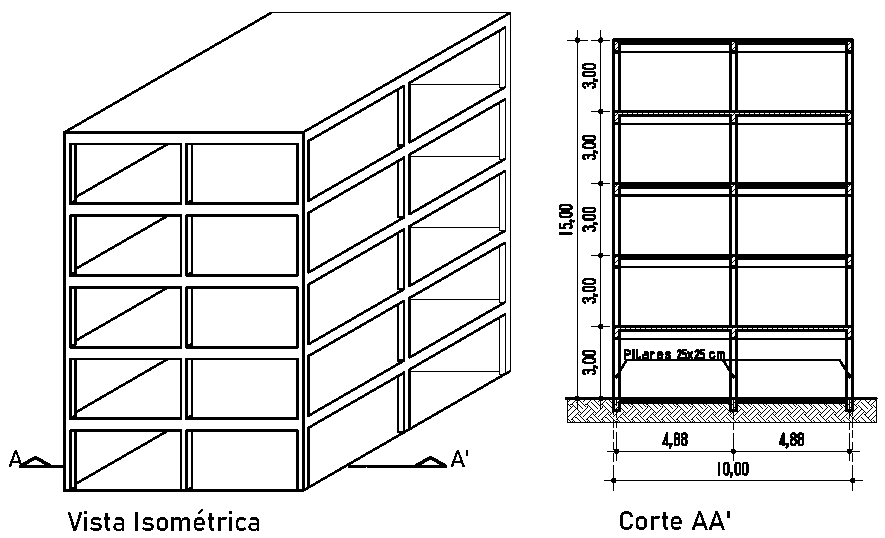
\includegraphics[scale=0.9]{../Images/VistaeCorte}
	\label{fig:edfestudo}
\end{figure}


Conforme Soriano (2014), a análise dinâmica de edifícios de múltiplos pavimentos pode ser realizada matematicamente com modelos de diferentes graus de refinamento. Esses modelos costumam ter suas massas concentradas nos pavimentos e podem ser do tipo \textit{shear building} ou tridimensionais.

O modelo \textit{shear building}, clássico e de grande simplicidade, supõe pisos indeformáveis e colunas inextensíveis. Matematicamente esse modelo equivale à uma coluna de trechos de rigidezes iguais à soma das rigidezes à flexão dos pilares de cada pavimento da edificação. No caso de edifícios com dois planos de simetria esse modelo pode ser plano, tendo apenas uma translação horizontal por pavimento (Soriano, 2014). Na figura \ref{fig:shearb} é apresentado um modelo plano de \textit{shear building} e o modelo matemático equivalente. 

\begin{figure}
	\centering
	\caption{Modelo \textit{shear building}.\\ \small{(Adaptado de Soriano, 2014)}}
	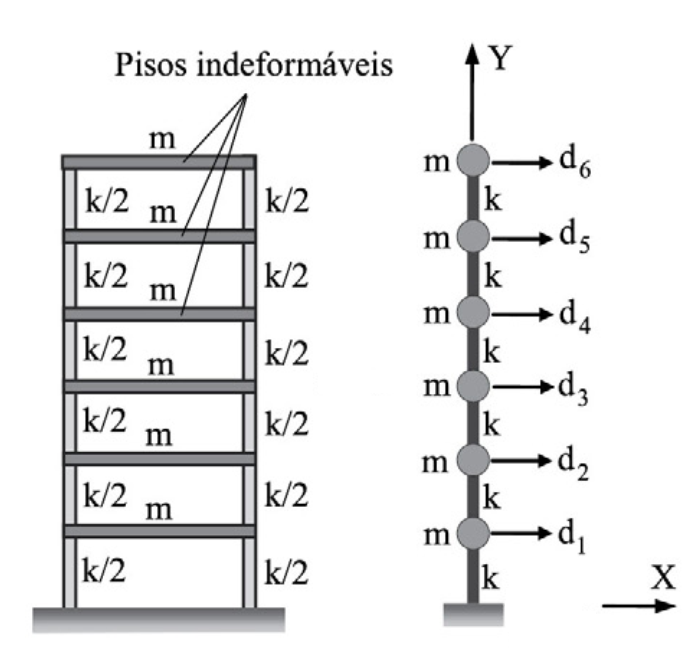
\includegraphics[scale=0.39]{../Images/ShearBuilding}
	\label{fig:shearb}
\end{figure}


Dessa forma, visando determinar a primeira frequência de vibração do edifício da figura \ref{fig:edfestudo}, o modelo reduzido construído será um modelo plano de \textit{shear building}. A frequência de vibração será determinada por meio das acelerações medidas no topo do modelo, através dessas também poderá ser determinado o amortecimento do modelo reduzido, para estudos posteriores. 


\section{Projeto do modelo reduzido}

    
    

    
    \begin{tcolorbox}[breakable, size=fbox, boxrule=1pt, pad at break*=1mm,colback=cellbackground, colframe=cellborder]
\prompt{In}{incolor}{1}{\boxspacing}
\begin{Verbatim}[commandchars=\\\{\}]
\PY{c+c1}{\PYZsh{} Importando e configurando módulos}
\PY{k+kn}{import} \PY{n+nn}{numpy} \PY{k}{as} \PY{n+nn}{np}
\PY{k+kn}{import} \PY{n+nn}{pandas} \PY{k}{as} \PY{n+nn}{pd} 
\PY{k+kn}{import} \PY{n+nn}{matplotlib}\PY{n+nn}{.}\PY{n+nn}{pyplot} \PY{k}{as} \PY{n+nn}{plt}
\PY{o}{\PYZpc{}}\PY{k}{config} InlineBackend.figure\PYZus{}format = \PYZsq{}svg\PYZsq{}
\PY{k+kn}{import} \PY{n+nn}{jupyter2latex} \PY{k}{as} \PY{n+nn}{j2l}
\PY{k+kn}{from} \PY{n+nn}{math} \PY{k+kn}{import} \PY{n}{pi}
\end{Verbatim}
\end{tcolorbox}



O projeto do modelo reduzido é baseado na introdução de escalas que
relacionem grandezas do modelo reduzido e do modelo real, onde o número
de escalas deve ser menor ou igual ao número de grandezas fundamentais
envolvidas no problema. Para o problema em questão as grandezas
fundamentais são três: comprimento (\(L\)), massa (\(M\)) e tempo
(\(T\)), que formam a base da matriz dimensional. Para construção do
modelo reduzido as grandezas escolhidas para serem escaladas são
relativas ao comprimento (\(L\)), à rigidez à flexão (\(EI\)) e à
aceleração (\(a\)).

    Os fatores de escala adotados para \(L\) e \(EI\) são baseados no
material empregado para construção das colunas do modelo, essas serão
formadas por réguas de alumínio, com cerca de \(50 cm\) de comprimento,
à serem adquiridas e caracterizadas. A distância entre os pavimentos
será representada por trechos de \(10 cm\), logo, a escala de
comprimento \(\lambda_L\) será:

    \begin{tcolorbox}[breakable, size=fbox, boxrule=1pt, pad at break*=1mm,colback=cellbackground, colframe=cellborder]
\prompt{In}{incolor}{2}{\boxspacing}
\begin{Verbatim}[commandchars=\\\{\}]
\PY{n}{L\PYZus{}pav} \PY{o}{=} \PY{l+m+mi}{10}
\PY{n}{scale\PYZus{}L} \PY{o}{=} \PY{n}{L\PYZus{}pav}\PY{o}{/}\PY{l+m+mi}{300}

\PY{n}{j2l}\PY{o}{.}\PY{n}{print}\PY{p}{(}\PY{l+s+sa}{f}\PY{l+s+s2}{\PYZdq{}}\PY{l+s+s2}{\PYZdl{}\PYZdl{} }\PY{l+s+s2}{\PYZbs{}}\PY{l+s+s2}{lambda\PYZus{}L = 1:}\PY{l+s+si}{\PYZob{}}\PY{l+m+mi}{1}\PY{o}{/}\PY{n}{scale\PYZus{}L}\PY{l+s+si}{:}\PY{l+s+s2}{.2f}\PY{l+s+si}{\PYZcb{}}\PY{l+s+s2}{ \PYZdl{}\PYZdl{}}\PY{l+s+s2}{\PYZdq{}}\PY{p}{)}
\end{Verbatim}
\end{tcolorbox}

    $$ \lambda_L = 1:30.00 $$

    
    A escala da rigidez à flexão \(EI\) relaciona a rigidez de 2 réguas às
colunas do edifício. Adotando concreto da classe C25 tem-se
\(E_C=28GPa\), enquanto para a régua em alumínio tem-se \(E_{r}=70GPa\).
Em relação às geometrias, são estimadas para às reguas larguras de
\(2.5cm\) e espessuras de \(0.1cm\), enquanto os pilares tem seção
quadrada de \(25 \times 25cm\); seus momentos de inércia \(I\) são dados
por \ref{eq:mI}.

\begin{equation}
\label{eq:mI}
I = \frac{bh^3}{12}
\end{equation}

Dessa forma:

    \begin{tcolorbox}[breakable, size=fbox, boxrule=1pt, pad at break*=1mm,colback=cellbackground, colframe=cellborder]
\prompt{In}{incolor}{3}{\boxspacing}
\begin{Verbatim}[commandchars=\\\{\}]
\PY{c+c1}{\PYZsh{} Propriedades dos materiais}
\PY{n}{E\PYZus{}C} \PY{o}{=} \PY{l+m+mf}{28E9}  \PY{c+c1}{\PYZsh{} Concreto}
\PY{n}{E\PYZus{}r} \PY{o}{=} \PY{l+m+mf}{70E9}  \PY{c+c1}{\PYZsh{} Régua}

\PY{c+c1}{\PYZsh{} Geometria em concreto dos pilares}
\PY{n}{b\PYZus{}C} \PY{o}{=} \PY{l+m+mf}{0.25}
\PY{n}{h\PYZus{}C} \PY{o}{=} \PY{l+m+mf}{0.25}
\PY{n}{I\PYZus{}C} \PY{o}{=} \PY{n}{b\PYZus{}C}\PY{o}{*}\PY{n}{h\PYZus{}C}\PY{o}{*}\PY{o}{*}\PY{l+m+mi}{3}\PY{o}{/}\PY{l+m+mi}{12}
\PY{n}{EI\PYZus{}C} \PY{o}{=} \PY{n}{E\PYZus{}C} \PY{o}{*} \PY{n}{I\PYZus{}C}
\PY{n}{j2l}\PY{o}{.}\PY{n}{print}\PY{p}{(}\PY{l+s+sa}{f}\PY{l+s+s1}{\PYZsq{}\PYZsq{}\PYZsq{}}\PY{l+s+s1}{\PYZhy{} Momento de inércia de um pilar em concreto: \PYZdl{}}\PY{l+s+si}{\PYZob{}}\PY{n}{I\PYZus{}C}\PY{l+s+si}{=:}\PY{l+s+s1}{.3E}\PY{l+s+si}{\PYZcb{}}\PY{l+s+s1}{ }\PY{l+s+s1}{\PYZbs{}}\PY{l+s+s1}{: m\PYZca{}4\PYZdl{}. }

\PY{l+s+s1}{\PYZhy{} Rigidez à flexão do pilar em concreto: \PYZdl{}}\PY{l+s+si}{\PYZob{}}\PY{n}{EI\PYZus{}C}\PY{l+s+si}{=:}\PY{l+s+s1}{.3E}\PY{l+s+si}{\PYZcb{}}\PY{l+s+s1}{ Nm\PYZca{}2\PYZdl{}}\PY{l+s+s1}{\PYZsq{}\PYZsq{}\PYZsq{}}\PY{p}{)}

\PY{c+c1}{\PYZsh{} Geometria da régua}
\PY{n}{b\PYZus{}r} \PY{o}{=} \PY{l+m+mf}{0.025}
\PY{n}{h\PYZus{}r} \PY{o}{=} \PY{l+m+mf}{0.001}
\PY{n}{I\PYZus{}r} \PY{o}{=} \PY{n}{b\PYZus{}r}\PY{o}{*}\PY{n}{h\PYZus{}r}\PY{o}{*}\PY{o}{*}\PY{l+m+mi}{3}\PY{o}{/}\PY{l+m+mi}{12}
\PY{n}{EI\PYZus{}r} \PY{o}{=} \PY{n}{E\PYZus{}r} \PY{o}{*} \PY{n}{I\PYZus{}r} 
\PY{n}{j2l}\PY{o}{.}\PY{n}{print}\PY{p}{(}\PY{l+s+sa}{f}\PY{l+s+s1}{\PYZsq{}\PYZsq{}\PYZsq{}}\PY{l+s+s1}{\PYZhy{} Momento de inércia de uma regua em alumínio: \PYZdl{}}\PY{l+s+si}{\PYZob{}}\PY{n}{I\PYZus{}r}\PY{l+s+si}{=:}\PY{l+s+s1}{.3E}\PY{l+s+si}{\PYZcb{}}\PY{l+s+s1}{ }\PY{l+s+s1}{\PYZbs{}}\PY{l+s+s1}{: m\PYZca{}4\PYZdl{}. }

\PY{l+s+s1}{\PYZhy{} Rigidez à flexão da régua em alumínio: \PYZdl{}}\PY{l+s+si}{\PYZob{}}\PY{n}{EI\PYZus{}r}\PY{l+s+si}{=:}\PY{l+s+s1}{.3E}\PY{l+s+si}{\PYZcb{}}\PY{l+s+s1}{ Nm\PYZca{}2\PYZdl{}}\PY{l+s+s1}{\PYZsq{}\PYZsq{}\PYZsq{}}\PY{p}{)}
\end{Verbatim}
\end{tcolorbox}

    - Momento de inércia de um pilar em concreto: $I_C=3.255E-04 \: m^4$. 

- Rigidez à flexão do pilar em concreto: $EI_C=9.115E+06 Nm^2$

    
    - Momento de inércia de uma regua em alumínio: $I_r=2.083E-12 \: m^4$. 

- Rigidez à flexão da régua em alumínio: $EI_r=1.458E-01 Nm^2$

    
    Conforme descrito anteriormente o edifício é composto por 9 pilares,
distribuídos em 3 linhas, enquanto o modelo em escala é composto por
duas réguas, dessa forma, a escala da rigidez à flexão \(\lambda_{EI}\)
será:

    \begin{tcolorbox}[breakable, size=fbox, boxrule=1pt, pad at break*=1mm,colback=cellbackground, colframe=cellborder]
\prompt{In}{incolor}{4}{\boxspacing}
\begin{Verbatim}[commandchars=\\\{\}]
\PY{n}{scale\PYZus{}EI} \PY{o}{=} \PY{p}{(}\PY{l+m+mi}{2}\PY{o}{*}\PY{n}{EI\PYZus{}r}\PY{p}{)} \PY{o}{/} \PY{p}{(}\PY{l+m+mi}{9}\PY{o}{*}\PY{n}{EI\PYZus{}C}\PY{p}{)}
\PY{n}{j2l}\PY{o}{.}\PY{n}{print}\PY{p}{(}\PY{l+s+s2}{\PYZdq{}}\PY{l+s+s2}{\PYZdl{}\PYZdl{} }\PY{l+s+s2}{\PYZbs{}}\PY{l+s+s2}{lambda\PYZus{}}\PY{l+s+si}{\PYZob{}EI\PYZcb{}}\PY{l+s+s2}{ =}\PY{l+s+s2}{\PYZdq{}} \PY{o}{+} \PY{l+s+sa}{f}\PY{l+s+s2}{\PYZdq{}}\PY{l+s+s2}{1:}\PY{l+s+si}{\PYZob{}}\PY{l+m+mi}{1}\PY{o}{/}\PY{n}{scale\PYZus{}EI}\PY{l+s+si}{:}\PY{l+s+s2}{.3E}\PY{l+s+si}{\PYZcb{}}\PY{l+s+s2}{\PYZdl{}\PYZdl{}}\PY{l+s+s2}{\PYZdq{}}\PY{p}{)}
\end{Verbatim}
\end{tcolorbox}

    $$ \lambda_{EI} =1:2.812E+08$$

    
    Em relação à escala de acelerações (\(a\)) optou-se inicialmente por
manter a proporção \(\lambda_a=1:1\). Todavia, visto que o problema de
vibração livre é independente da aceleração da gravidade essa poderá ser
alterada de forma a facilitar a construção do modelo.

    \begin{tcolorbox}[breakable, size=fbox, boxrule=1pt, pad at break*=1mm,colback=cellbackground, colframe=cellborder]
\prompt{In}{incolor}{5}{\boxspacing}
\begin{Verbatim}[commandchars=\\\{\}]
\PY{n}{scale\PYZus{}a} \PY{o}{=} \PY{l+m+mi}{1}\PY{o}{/}\PY{l+m+mi}{1}
\end{Verbatim}
\end{tcolorbox}

    Em posse das escalas impostas, para construção do modelo reduzido e
realização da análise devem ser conhecidas as escalas derivadas
necessárias, que são obtidas através de uma análise dimensional, onde a
base da nova matriz dimensional será formada pelas grandezas \(L\),
\(EI\) e \(a\). Fazendo uso da metodologia implementada por Rocha
(2020), a base da matriz dimensional é alterada para a base \(L\),
\(EI\) e \(a\):

    \begin{tcolorbox}[breakable, size=fbox, boxrule=1pt, pad at break*=1mm,colback=cellbackground, colframe=cellborder]
\prompt{In}{incolor}{6}{\boxspacing}
\begin{Verbatim}[commandchars=\\\{\}]
\PY{c+c1}{\PYZsh{} Importando DimData }
\PY{n}{DimData} \PY{o}{=} \PY{n}{pd}\PY{o}{.}\PY{n}{read\PYZus{}excel}\PY{p}{(}\PY{l+s+s1}{\PYZsq{}}\PY{l+s+s1}{../Resources/DimData.xlsx}\PY{l+s+s1}{\PYZsq{}}\PY{p}{,} \PY{n}{index\PYZus{}col}\PY{o}{=}\PY{l+m+mi}{0}\PY{p}{,} \PY{n}{sheet\PYZus{}name}\PY{o}{=}\PY{l+s+s1}{\PYZsq{}}\PY{l+s+s1}{DimData}\PY{l+s+s1}{\PYZsq{}}\PY{p}{)}

\PY{c+c1}{\PYZsh{} Grandezas fundamentais originais }
\PY{n}{LMT} \PY{o}{=} \PY{p}{[}\PY{l+s+s1}{\PYZsq{}}\PY{l+s+s1}{L}\PY{l+s+s1}{\PYZsq{}}\PY{p}{,} \PY{l+s+s1}{\PYZsq{}}\PY{l+s+s1}{M}\PY{l+s+s1}{\PYZsq{}}\PY{p}{,} \PY{l+s+s1}{\PYZsq{}}\PY{l+s+s1}{T}\PY{l+s+s1}{\PYZsq{}}\PY{p}{]}

\PY{c+c1}{\PYZsh{} Novas base de grandezas}
\PY{n}{ABC} \PY{o}{=} \PY{p}{[}\PY{l+s+s1}{\PYZsq{}}\PY{l+s+s1}{L}\PY{l+s+s1}{\PYZsq{}}\PY{p}{,} \PY{l+s+s1}{\PYZsq{}}\PY{l+s+s1}{EI}\PY{l+s+s1}{\PYZsq{}}\PY{p}{,} \PY{l+s+s1}{\PYZsq{}}\PY{l+s+s1}{a}\PY{l+s+s1}{\PYZsq{}}\PY{p}{]} 

\PY{c+c1}{\PYZsh{} Importa matriz dimensional de ABC na base LMT}
\PY{n}{base} \PY{o}{=} \PY{n}{DimData}\PY{o}{.}\PY{n}{loc}\PY{p}{[}\PY{n}{ABC}\PY{p}{,} \PY{n}{LMT}\PY{p}{]}
\PY{n}{j2l}\PY{o}{.}\PY{n}{df2table}\PY{p}{(}\PY{n}{base}\PY{p}{,} \PY{l+s+s1}{\PYZsq{}}\PY{l+s+si}{\PYZob{}\PYZcb{}}\PY{l+s+s1}{ na base }\PY{l+s+si}{\PYZob{}\PYZcb{}}\PY{l+s+s1}{\PYZsq{}}\PY{o}{.}\PY{n}{format}\PY{p}{(}\PY{l+s+s1}{\PYZsq{}}\PY{l+s+s1}{,}\PY{l+s+s1}{\PYZsq{}}\PY{o}{.}\PY{n}{join}\PY{p}{(}\PY{n}{ABC}\PY{p}{)}\PY{p}{,} \PY{l+s+s1}{\PYZsq{}}\PY{l+s+s1}{,}\PY{l+s+s1}{\PYZsq{}}\PY{o}{.}\PY{n}{join}\PY{p}{(}\PY{n}{LMT}\PY{p}{)}\PY{p}{)}\PY{p}{)}

\PY{c+c1}{\PYZsh{} Inverte base de unidades de LMT para ABC}
\PY{n}{base\PYZus{}i} \PY{o}{=} \PY{n}{pd}\PY{o}{.}\PY{n}{DataFrame}\PY{p}{(}\PY{n}{np}\PY{o}{.}\PY{n}{linalg}\PY{o}{.}\PY{n}{inv}\PY{p}{(}\PY{n}{base}\PY{p}{)}\PY{p}{,} \PY{n}{index}\PY{o}{=}\PY{n}{LMT}\PY{p}{,} \PY{n}{columns}\PY{o}{=}\PY{n}{ABC}\PY{p}{)}
\PY{n}{j2l}\PY{o}{.}\PY{n}{df2table}\PY{p}{(}\PY{n}{base\PYZus{}i}\PY{p}{,} \PY{l+s+s1}{\PYZsq{}}\PY{l+s+si}{\PYZob{}\PYZcb{}}\PY{l+s+s1}{ na base }\PY{l+s+si}{\PYZob{}\PYZcb{}}\PY{l+s+s1}{\PYZsq{}}\PY{o}{.}\PY{n}{format}\PY{p}{(}\PY{l+s+s1}{\PYZsq{}}\PY{l+s+s1}{,}\PY{l+s+s1}{\PYZsq{}}\PY{o}{.}\PY{n}{join}\PY{p}{(}\PY{n}{LMT}\PY{p}{)}\PY{p}{,} \PY{l+s+s1}{\PYZsq{}}\PY{l+s+s1}{,}\PY{l+s+s1}{\PYZsq{}}\PY{o}{.}\PY{n}{join}\PY{p}{(}\PY{n}{ABC}\PY{p}{)}\PY{p}{)}\PY{p}{)}
\end{Verbatim}
\end{tcolorbox}

    
    \begin{table}[H]
    \centering
    \caption{L,EI,a na base L,M,T}
    {\begin{tabular}{lrrr}
\toprule
{} &  L &  M &  T \\
\midrule
L  &  1 &  0 &  0 \\
EI &  3 &  1 & -2 \\
a  &  1 &  0 & -2 \\
\bottomrule
\end{tabular}
}
    \label{}
    \end{table}
    

    
    
    \begin{table}[H]
    \centering
    \caption{L,M,T na base L,EI,a}
    {\begin{tabular}{lrrr}
\toprule
{} &    L &   EI &    a \\
\midrule
L &  1.0 &  0.0 &  0.0 \\
M & -2.0 &  1.0 & -1.0 \\
T &  0.5 & -0.0 & -0.5 \\
\bottomrule
\end{tabular}
}
    \label{}
    \end{table}
    

    
    Para análise do modelo reduzido é necessário o conhecimento da escala de
massa (\(\lambda_m\)), necessária para determinação das massas dos
pavimentos, e a escala de frequências (\(\lambda_f\)), que relaciona as
frequências de vibração do modelo reduzido e da estrutura real. Para a
determinação da tais fatores essas grandezas devem estar presentes na
matriz dimensional de base \(L\), \(EI\) e \(a\).

    \begin{tcolorbox}[breakable, size=fbox, boxrule=1pt, pad at break*=1mm,colback=cellbackground, colframe=cellborder]
\prompt{In}{incolor}{7}{\boxspacing}
\begin{Verbatim}[commandchars=\\\{\}]
\PY{n}{par} \PY{o}{=} \PY{n}{ABC} \PY{o}{+} \PY{p}{[}\PY{l+s+s1}{\PYZsq{}}\PY{l+s+s1}{m}\PY{l+s+s1}{\PYZsq{}}\PY{p}{,} \PY{l+s+s1}{\PYZsq{}}\PY{l+s+s1}{f}\PY{l+s+s1}{\PYZsq{}}\PY{p}{]}
\PY{n}{npar} \PY{o}{=} \PY{n+nb}{len}\PY{p}{(}\PY{n}{par}\PY{p}{)}

\PY{n}{DMat\PYZus{}LMT} \PY{o}{=} \PY{n}{DimData}\PY{o}{.}\PY{n}{loc}\PY{p}{[}\PY{n}{par}\PY{p}{,} \PY{n}{LMT}\PY{p}{]}
\PY{n}{DMat\PYZus{}ABC} \PY{o}{=} \PY{n}{np}\PY{o}{.}\PY{n}{matmul}\PY{p}{(}\PY{n}{DMat\PYZus{}LMT}\PY{p}{,} \PY{n}{base\PYZus{}i}\PY{p}{)}
\PY{n}{DMat\PYZus{}ABC}\PY{o}{.}\PY{n}{rename}\PY{p}{(}\PY{n}{columns}\PY{o}{=}\PY{n+nb}{dict}\PY{p}{(}\PY{n+nb}{zip}\PY{p}{(}\PY{n}{LMT}\PY{p}{,} \PY{n}{ABC}\PY{p}{)}\PY{p}{)}\PY{p}{,} \PY{n}{inplace}\PY{o}{=}\PY{k+kc}{True}\PY{p}{)} \PY{c+c1}{\PYZsh{} Renomeia colunas para nova base}
\PY{n}{j2l}\PY{o}{.}\PY{n}{df2table}\PY{p}{(}\PY{n}{DMat\PYZus{}ABC}\PY{p}{,} \PY{l+s+s1}{\PYZsq{}}\PY{l+s+s1}{Matriz \PYZdl{}D\PYZdl{}  na base }\PY{l+s+si}{\PYZob{}\PYZcb{}}\PY{l+s+s1}{\PYZsq{}}\PY{o}{.}\PY{n}{format}\PY{p}{(}\PY{l+s+s1}{\PYZsq{}}\PY{l+s+s1}{,}\PY{l+s+s1}{\PYZsq{}}\PY{o}{.}\PY{n}{join}\PY{p}{(}\PY{n}{ABC}\PY{p}{)}\PY{p}{)}\PY{p}{)}
\end{Verbatim}
\end{tcolorbox}

    
    \begin{table}[H]
    \centering
    \caption{Matriz $D$  na base L,EI,a}
    {\begin{tabular}{lrrr}
\toprule
{} &    L &   EI &    a \\
\midrule
L  &  1.0 &  0.0 &  0.0 \\
EI &  0.0 &  1.0 &  0.0 \\
a  &  0.0 &  0.0 &  1.0 \\
m  & -2.0 &  1.0 & -1.0 \\
f  & -0.5 &  0.0 &  0.5 \\
\bottomrule
\end{tabular}
}
    \label{}
    \end{table}
    

    
    Por fim, aplicando sobre a matriz \(\bf{D}\) as escalas impostas tem-se
a tabela de escalas:

    \begin{tcolorbox}[breakable, size=fbox, boxrule=1pt, pad at break*=1mm,colback=cellbackground, colframe=cellborder]
\prompt{In}{incolor}{8}{\boxspacing}
\begin{Verbatim}[commandchars=\\\{\}]
\PY{n}{escalas} \PY{o}{=} \PY{n}{np}\PY{o}{.}\PY{n}{array}\PY{p}{(}\PY{p}{[}\PY{n}{scale\PYZus{}L}\PY{p}{,} \PY{n}{scale\PYZus{}EI}\PY{p}{,} \PY{n}{scale\PYZus{}a}\PY{p}{]}\PY{p}{)}
\PY{n}{escalas} \PY{o}{=} \PY{n}{np}\PY{o}{.}\PY{n}{tile}\PY{p}{(}\PY{n}{escalas}\PY{p}{,} \PY{p}{(}\PY{n}{npar}\PY{p}{,} \PY{l+m+mi}{1}\PY{p}{)}\PY{p}{)}
\PY{n}{escalas} \PY{o}{=} \PY{n}{np}\PY{o}{.}\PY{n}{prod}\PY{p}{(}\PY{n}{escalas}\PY{o}{*}\PY{o}{*}\PY{n}{DMat\PYZus{}ABC}\PY{p}{,} \PY{n}{axis}\PY{o}{=}\PY{l+m+mi}{1}\PY{p}{)}
\PY{n}{escalas} \PY{o}{=} \PY{n}{pd}\PY{o}{.}\PY{n}{DataFrame}\PY{p}{(}\PY{p}{\PYZob{}}\PY{l+s+s1}{\PYZsq{}}\PY{l+s+s1}{λ}\PY{l+s+s1}{\PYZsq{}}\PY{p}{:} \PY{n}{escalas}\PY{p}{,} \PY{l+s+s1}{\PYZsq{}}\PY{l+s+s1}{1/λ}\PY{l+s+s1}{\PYZsq{}}\PY{p}{:} \PY{l+m+mi}{1}\PY{o}{/}\PY{n}{escalas}\PY{p}{\PYZcb{}}\PY{p}{,} \PY{n}{index}\PY{o}{=}\PY{n}{par}\PY{p}{)}
\PY{n}{j2l}\PY{o}{.}\PY{n}{df2table}\PY{p}{(}\PY{n}{escalas}\PY{p}{,} \PY{l+s+s1}{\PYZsq{}}\PY{l+s+s1}{Fatores de escala}\PY{l+s+s1}{\PYZsq{}}\PY{p}{)}

\PY{n}{j2l}\PY{o}{.}\PY{n}{print}\PY{p}{(}\PY{l+s+s2}{\PYZdq{}\PYZdq{}\PYZdq{}}\PY{l+s+s2}{Escalas derivadas:}

\PY{l+s+s2}{\PYZhy{} Escala de massa: \PYZdl{}}\PY{l+s+s2}{\PYZbs{}}\PY{l+s+s2}{lambda\PYZus{}m = 1:}\PY{l+s+si}{\PYZob{}:.2E\PYZcb{}}\PY{l+s+s2}{\PYZdl{}}

\PY{l+s+s2}{\PYZhy{} Escala de frequências: \PYZdl{}}\PY{l+s+s2}{\PYZbs{}}\PY{l+s+s2}{lambda\PYZus{}f = }\PY{l+s+si}{\PYZob{}:.3f\PYZcb{}}\PY{l+s+s2}{:1\PYZdl{}}\PY{l+s+s2}{\PYZdq{}\PYZdq{}\PYZdq{}}\PY{o}{.}\PY{n}{format}\PY{p}{(}\PY{n}{escalas}\PY{o}{.}\PY{n}{loc}\PY{p}{[}\PY{l+s+s1}{\PYZsq{}}\PY{l+s+s1}{m}\PY{l+s+s1}{\PYZsq{}}\PY{p}{,} \PY{l+s+s1}{\PYZsq{}}\PY{l+s+s1}{1/λ}\PY{l+s+s1}{\PYZsq{}}\PY{p}{]}\PY{p}{,} \PY{n}{escalas}\PY{o}{.}\PY{n}{loc}\PY{p}{[}\PY{l+s+s1}{\PYZsq{}}\PY{l+s+s1}{f}\PY{l+s+s1}{\PYZsq{}}\PY{p}{,} \PY{l+s+s1}{\PYZsq{}}\PY{l+s+s1}{λ}\PY{l+s+s1}{\PYZsq{}}\PY{p}{]}\PY{p}{)}\PY{p}{)}
\end{Verbatim}
\end{tcolorbox}

    
    \begin{table}[H]
    \centering
    \caption{Fatores de escala}
    {\begin{tabular}{lrr}
\toprule
{} &             λ &           1/λ \\
\midrule
L  &  3.333333e-02 &  3.000000e+01 \\
EI &  3.555556e-09 &  2.812500e+08 \\
a  &  1.000000e+00 &  1.000000e+00 \\
m  &  3.200000e-06 &  3.125000e+05 \\
f  &  5.477226e+00 &  1.825742e-01 \\
\bottomrule
\end{tabular}
}
    \label{}
    \end{table}
    

    
    Escalas derivadas:

- Escala de massa: $\lambda_m = 1:3.12E+05$

- Escala de frequências: $\lambda_f = 5.477:1$

    
    Dessa forma a massa dos pavimentos do modelo em escala devem ter
\(1/312500\) da massa de cada pavimento da estrutura real. Sendo que as
vigas tem seção \(25\times50 cm\), a laje tem \(h=10cm\) e considerando
uma carga permanente (alvenarias, revestimentos e etc.) de
\(300 kg/m^2\) sobre todos os pavimentos, a massa dos pavimentos são:

    \begin{tcolorbox}[breakable, size=fbox, boxrule=1pt, pad at break*=1mm,colback=cellbackground, colframe=cellborder]
\prompt{In}{incolor}{9}{\boxspacing}
\begin{Verbatim}[commandchars=\\\{\}]
\PY{n}{M\PYZus{}vigas}   \PY{o}{=} \PY{l+m+mf}{0.25}\PY{o}{*}\PY{l+m+mf}{0.50} \PY{o}{*} \PY{l+m+mi}{10} \PY{o}{*} \PY{l+m+mi}{6} \PY{o}{*} \PY{l+m+mi}{2500}   \PY{c+c1}{\PYZsh{} 6 vigas de 10 metros por pavimento}
\PY{n}{M\PYZus{}laje}    \PY{o}{=} \PY{l+m+mf}{0.10} \PY{o}{*} \PY{l+m+mi}{10}\PY{o}{*}\PY{l+m+mi}{10} \PY{o}{*} \PY{l+m+mi}{2500}         \PY{c+c1}{\PYZsh{} Laje 10x10 e h=12cm}
\PY{n}{M\PYZus{}cargas}  \PY{o}{=} \PY{l+m+mi}{300} \PY{o}{*} \PY{l+m+mi}{10}\PY{o}{*}\PY{l+m+mi}{10}                 \PY{c+c1}{\PYZsh{} carga de 300 kg/m²}
\PY{n}{M\PYZus{}pilares} \PY{o}{=} \PY{l+m+mf}{0.25}\PY{o}{*}\PY{o}{*}\PY{l+m+mi}{2} \PY{o}{*} \PY{l+m+mi}{3} \PY{o}{*} \PY{l+m+mi}{2500} \PY{o}{*} \PY{l+m+mi}{9}      \PY{c+c1}{\PYZsh{} 9 pilares de 3m por pavimento (1.5m apenas no pav superior)}

\PY{n}{M\PYZus{}pavtipo} \PY{o}{=} \PY{n}{M\PYZus{}vigas} \PY{o}{+} \PY{n}{M\PYZus{}laje} \PY{o}{+} \PY{n}{M\PYZus{}cargas} \PY{o}{+} \PY{n}{M\PYZus{}pilares}
\PY{n}{M\PYZus{}pavcob}  \PY{o}{=} \PY{n}{M\PYZus{}vigas} \PY{o}{+} \PY{n}{M\PYZus{}laje} \PY{o}{+} \PY{n}{M\PYZus{}cargas} \PY{o}{+} \PY{n}{M\PYZus{}pilares}\PY{o}{/}\PY{l+m+mi}{2}

\PY{n}{j2l}\PY{o}{.}\PY{n}{print}\PY{p}{(}\PY{l+s+s2}{\PYZdq{}\PYZdq{}\PYZdq{}}\PY{l+s+s2}{Massas da estrutura:}

\PY{l+s+s2}{\PYZhy{} Massa dos pavimentos tipo: }\PY{l+s+si}{\PYZob{}:.1f\PYZcb{}}

\PY{l+s+s2}{\PYZhy{} Massa do pavimento de cobertura }\PY{l+s+si}{\PYZob{}:.1f\PYZcb{}}\PY{l+s+s2}{\PYZdq{}\PYZdq{}\PYZdq{}}\PY{o}{.}\PY{n}{format}\PY{p}{(}\PY{n}{M\PYZus{}pavtipo}\PY{p}{,} \PY{n}{M\PYZus{}pavcob}\PY{p}{)}\PY{p}{)}
\end{Verbatim}
\end{tcolorbox}

    Massas da estrutura:

- Massa dos pavimentos tipo: 77968.8

- Massa do pavimento de cobertura 75859.4

    
    Logo as massas dos pavimentos do modelo em escala deverão ser:

    \begin{tcolorbox}[breakable, size=fbox, boxrule=1pt, pad at break*=1mm,colback=cellbackground, colframe=cellborder]
\prompt{In}{incolor}{10}{\boxspacing}
\begin{Verbatim}[commandchars=\\\{\}]
\PY{n}{j2l}\PY{o}{.}\PY{n}{print}\PY{p}{(}\PY{l+s+s2}{\PYZdq{}\PYZdq{}\PYZdq{}}
\PY{l+s+s2}{Massas do modelo em escala:}

\PY{l+s+s2}{\PYZhy{} Massa dos pavimentos tipo: }\PY{l+s+si}{\PYZob{}:.3f\PYZcb{}}

\PY{l+s+s2}{\PYZhy{} Massa do pavimento de cobertura }\PY{l+s+si}{\PYZob{}:.3f\PYZcb{}}\PY{l+s+s2}{\PYZdq{}\PYZdq{}\PYZdq{}}\PY{o}{.}\PY{n}{format}\PY{p}{(}\PY{n}{M\PYZus{}pavtipo}\PY{o}{*}\PY{n}{escalas}\PY{o}{.}\PY{n}{loc}\PY{p}{[}\PY{l+s+s1}{\PYZsq{}}\PY{l+s+s1}{m}\PY{l+s+s1}{\PYZsq{}}\PY{p}{,} \PY{l+s+s1}{\PYZsq{}}\PY{l+s+s1}{λ}\PY{l+s+s1}{\PYZsq{}}\PY{p}{]}\PY{p}{,} \PY{n}{M\PYZus{}pavcob}\PY{o}{*}\PY{n}{escalas}\PY{o}{.}\PY{n}{loc}\PY{p}{[}\PY{l+s+s1}{\PYZsq{}}\PY{l+s+s1}{m}\PY{l+s+s1}{\PYZsq{}}\PY{p}{,} \PY{l+s+s1}{\PYZsq{}}\PY{l+s+s1}{λ}\PY{l+s+s1}{\PYZsq{}}\PY{p}{]}\PY{p}{)}\PY{p}{)}
\end{Verbatim}
\end{tcolorbox}

    
Massas do modelo em escala:

- Massa dos pavimentos tipo: 0.250

- Massa do pavimento de cobertura 0.243

    





\section{Referências Bibliográficas}

Rocha, M. M. \textbf{PEC00144 - Experimental Methods in Civil Engineering}, 2020. 
Disponível em: \url{https://github.com/mmaiarocha/PEC00144}.

Soriano, H. L. \textbf{Introdução à dinâmica das estruturas}. Rio de Janeiro: Elsevier, 2014.

    
\end{document}


